\documentclass{article}
\usepackage[
  margin = 1in,
]{geometry}
\usepackage{amsmath, amssymb}
\usepackage{enumitem}
\usepackage{bm}
\usepackage{tikz}

\begin{document}
\section*{Problem}
\begin{enumerate}[label=\fbox{\arabic*}]
  \item Determine all possible groups $G$ satisfying both of the following conditions.
        \begin{description}
          \item[(Condition 1)] $G$ is a finite abelian group.
          \item[(Condition 2)] $G$ is isomorphic to a subgroup of $\mathrm{SL}_2(\mathbb{Z})$.
        \end{description}
        Here $\mathrm{SL}_2(\mathbb{Z})$ is the group of $2 \times 2$ matrices whose entries are integers and whose determinant is 1.

  \item Prove that every maximal ideal of the polynomial ring $\mathbb{R}[X, Y]$ of two variables over $\mathbb{R}$ has one of the following forms.
        \begin{itemize}
          \item $(X + a, Y + b) \quad (a, b \in \mathbb{R})$
          \item $(X^2 + aX + b, Y + cX + d) \quad (a, b, c, d \in \mathbb{R})$
          \item $(X + aY + b, Y^2 + cY + d) \quad (a, b, c, d \in \mathbb{R})$
        \end{itemize}

  \item For a positive integer $n$, define a polynomial $f_n(X)$ with integer coefficients as follows.
        \[
          \begin{cases}
            f_1(X) = X^2 - 2 \\
            f_n(X) = f_{n-1}(X^2 - 2) & (n \ge 2)
          \end{cases}
        \]
        Let $K_n$ be the smallest splitting field of $f_n(X)$ over $\mathbb{Q}$. Calculate the Galois group $\mathrm{Gal}(K_n/\mathbb{Q})$.

  \item We define a subset $M$ of $\mathbb{R}^3 \setminus \{(0, 0, 0)\}$ by
        \[
          M = \{ (x, y, z) \in \mathbb{R}^3 \setminus \{(0, 0, 0)\} \mid x^2 + y^2 - z^2 + z^3 + z^4 = 0 \}.
        \]
        \begin{enumerate}[label=(\arabic*)]
          \item Prove that $M$ is a $C^\infty$-submanifold of $\mathbb{R}^3 \setminus \{(0, 0, 0)\}$.
          \item We define a map $f: M \to S^2$ by
                \[
                  f(x, y, z) = \frac{1}{\sqrt{x^2 + y^2 + z^2}} (x, y, z),
                \]
                where $S^2 = \{ (x, y, z) \in \mathbb{R}^3 \mid x^2 + y^2 + z^2 = 1 \}$.
                Find the set of critical values of $f$.
        \end{enumerate}

  \item We set $S^6 = \{ (x_1, x_2, x_3, x_4, x_5, x_6, x_7) \in \mathbb{R}^7 \mid x_1^2 + x_2^2 + x_3^2 + \cdots + x_7^2 = 1 \}$. We define subsets $A, B$ of $S^6$ by
        \begin{align*}
          A &= \{ (x_1, x_2, x_3, x_4, x_5, x_6, x_7) \in S^6 \mid x_5 = x_6 = x_7 = 0 \} \\
          B &= \{ (x_1, x_2, x_3, x_4, x_5, x_6, x_7) \in S^6 \mid x_1 = x_2 = x_3 = 0 \}.
        \end{align*}
        \begin{enumerate}[label=(\arabic*)]
          \item Compute the homology groups of $S^6 \setminus A$ with integer coefficients.
          \item Compute the homology groups of $S^6 \setminus (A \cup B)$ with integer coefficients.
        \end{enumerate}

  \item Let $f$ be a real-valued Lebesgue measurable function on $\mathbb{R}$ such that
        \[
          \int_{\mathbb{R}} |f(x)|^2 \, dx < \infty, \quad \sup_{n \in \mathbb{N}} n^2 \int_{\mathbb{R}} |f(x) - f(n + x)|^2 \, dx < \infty,
        \]
        where $\mathbb{N}$ is the set of all nonnegative integers. Prove that
        \[
          \lim_{n \in \mathbb{N}, n \to \infty} f(n + x) = 0
        \]
        for almost every $x \in \mathbb{R}$.

  \item Let $L^2(\mathbb{R})$ be the Hilbert space of all square-integrable real-valued functions on $\mathbb{R}$, and define the norm of $f \in L^2(\mathbb{R})$ by
        \[
          \|f\| = \left( \int_{\mathbb{R}} |f(x)|^2 \, dx \right)^{\frac{1}{2}}.
        \]
        Answer the following questions.
        \begin{enumerate}[label=(\arabic*)]
          \item For $f \in L^2(\mathbb{R})$, set
                \[
                  (Tf)(x) = \int_{\mathbb{R}} e^{-(x-y)^2} f(y) \, dy.
                \]
                Prove that $T$ is a bounded operator on $L^2(\mathbb{R})$.
          \item Let $\varphi$ be a bounded $C^1$-function on $\mathbb{R}$ such that the derivative $\varphi'$ of $\varphi$ satisfies $\varphi' \in L^2(\mathbb{R})$, and define a bounded operator $S$ on $L^2(\mathbb{R})$ by
                \[
                  (Sf)(x) = \varphi(x) f(x).
                \]
                Prove that $ST - TS$ is a compact operator.
        \end{enumerate}

  \item Let $L^2(\mathbb{R}^3)$ be the Hilbert space of all square-integrable real-valued functions on $\mathbb{R}^3$.
        \begin{enumerate}[label=(\arabic*)]
          \item For a pair $f, g$ of rapidly decreasing real-valued functions on $\mathbb{R}^3$, set
                \[
                  B[f, g] = - \int_{\mathbb{R}^3} f(x) x \cdot \nabla g(x) \, dx,
                \]
                where $x \cdot \nabla = \sum_{j=1}^3 x_j \partial_{x_j}$. Prove that $B[f, f] \ge 0$.
          \item Assume that two sequences $\{f_n\}_{n=1}^\infty$ and $\{h_n\}_{n=1}^\infty$ of rapidly decreasing real-valued functions on $\mathbb{R}^3$ satisfy the following (a) and (b).
                \begin{enumerate}[label=(\alph*)]
                  \item There exists $h \in L^2(\mathbb{R}^3)$ such that $\{h_n\}_{n=1}^\infty$ converges to $h$ weakly in $L^2(\mathbb{R}^3)$.
                  \item For all rapidly decreasing real-valued function $\varphi$ on $\mathbb{R}^3$, it holds that
                        \[
                          \int_{\mathbb{R}^3} f_n(x) (|x|^2 \varphi(x) - \Delta \varphi(x)) \, dx = \int_{\mathbb{R}^3} h_n(x) \varphi(x) \, dx,
                        \]
                        where $\Delta = \sum_{j=1}^3 \partial_{x_j}^2$.
                \end{enumerate}
                Answer the following questions.
                \begin{enumerate}[label=(\roman*)]
                  \item Prove that there exists $f \in L^2(\mathbb{R}^3)$ satisfying the following (a') and (b').
                        \begin{enumerate}[label=(a')]
                          \item $f$ is a weak limit in $L^2(\mathbb{R}^3)$ of some subsequence $\{f_{n(k)}\}_{k=1}^\infty$ of $\{f_n\}_{n=1}^\infty$.
                          \item[(b')] For all rapidly decreasing real-valued function $\varphi$ on $\mathbb{R}^3$, it holds that
                                \[
                                  \int_{\mathbb{R}^3} f(x) (|x|^2 \varphi(x) - \Delta \varphi(x)) \, dx = \int_{\mathbb{R}^3} h(x) \varphi(x) \, dx.
                                \]
                        \end{enumerate}
                  \item Let $f$ be the function in (i). Prove that $|x|^2 f \in L^2(\mathbb{R}^3)$.
                \end{enumerate}
        \end{enumerate}

  \item Let $a > \frac{1}{2}$ and consider a system of ordinary differential equations for a function $(x(t), y(t)) \in \mathbb{R}^2$ of $t \in \mathbb{R}$
        \begin{equation*}
          \begin{cases}
            \dot{x} = x(a - x^2 - y^2) - y(1 + x + y) \\
            \dot{y} = x(1 + x + y) + y(a - x^2 - y^2),
          \end{cases} \tag{$*$}
        \end{equation*}
        where the dot "$\cdot$" means the differentiation with respect to $t$. Define $E_1, E_2 \in \mathbb{R}^2$ by
        \begin{align*}
          E_1 &= \left( \frac{-1 - \sqrt{2a - 1}}{2}, \frac{-1 + \sqrt{2a - 1}}{2} \right), \\
          E_2 &= \left( \frac{-1 + \sqrt{2a - 1}}{2}, \frac{-1 - \sqrt{2a - 1}}{2} \right).
        \end{align*}
        Answer the following questions.
        \begin{enumerate}[label=(\arabic*)]
          \item Prove that the circle centered at the origin with radius $\sqrt{a}$ is an invariant set of $(*)$.
          \item Prove the existence of a heteroclinic solution from the equilibrium point $E_2$ to the equilibrium point $E_1$.
          \item Prove the existence of a heteroclinic solution from the equilibrium point $(0, 0)$ to the equilibrium point $E_1$, and a heteroclinic solution from the equilibrium point $(0, 0)$ to the equilibrium point $E_2$.
        \end{enumerate}
        Here, for two different equilibrium points $p, q \in \mathbb{R}^2$ of $(*)$, we call a solution $(x(t), y(t))$ of $(*)$ a heteroclinic solution from $p$ to $q$ if $(x(t), y(t))$ satisfies
        \[
          \lim_{t \to -\infty} (x(t), y(t)) = p, \quad \lim_{t \to \infty} (x(t), y(t)) = q.
        \]

  \item We consider an incompressible viscous fluid between two parallel planes in a rotating frame of reference. The motion of fluid is driven by spatially-homogeneous constant pressure gradient force which is parallel to the planes. As depicted in the figure below, the planes are perpendicular to the axis of rotation of the system and we set this axis as our $z$ axis. The $x$ axis is taken in the direction of the pressure gradient force and the $y$ axis is taken to be perpendicular to these two axes.

        \begin{center}
        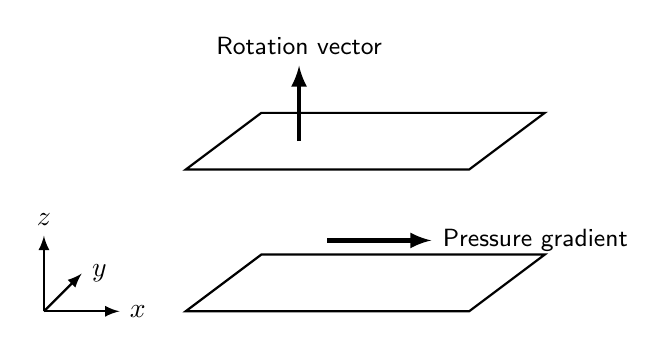
\begin{tikzpicture}[scale=1.2, >=latex]
          % Axes
          \begin{scope}[shift={(0, 0)}]
            \draw[->, thick] (0,0) -- (0.8,0) node[right] {$x$};
            \draw[->, thick] (0,0) -- (0,0.8) node[above] {$z$};
            \draw[->, thick] (0,0) -- (0.4,0.4) node[right] {$y$};
          \end{scope}
          
          % Bottom plane
          \draw[thick] (1.5, 0) -- (4.5, 0) -- (5.3, 0.6) -- (2.3, 0.6) -- cycle;
          
          % Top plane
          \draw[thick] (1.5, 1.5) -- (4.5, 1.5) -- (5.3, 2.1) -- (2.3, 2.1) -- cycle;
          
          % Rotation vector arrow
          \draw[->, ultra thick] (2.7, 1.8) -- (2.7, 2.6) node[above, font=\sffamily\small] {Rotation vector};
          
          % Pressure gradient arrow
          \draw[->, ultra thick] (3.0, 0.75) -- (4.1, 0.75) node[right, font=\sffamily\small] {Pressure gradient};
        \end{tikzpicture}
        \end{center}

        The two-dimensional fluid motion in the two parallel planes is governed by
        \begin{equation}
          -2\Omega v_* = \nu \frac{d^2 u_*}{dz_*^2} + F, \quad 2\Omega u_* = \nu \frac{d^2 v_*}{dz_*^2}, \quad u_*\left(\pm\frac{D}{2}\right) = v_*\left(\pm\frac{D}{2}\right) = 0, \tag{1}
        \end{equation}
        where $u_*(z_*)$ and $v_*(z_*)$ denote the $x$ and $y$ components of the fluid velocity at $z = z_*$, and positive constants, $\nu$, $F$, $D$, $\Omega$, the fluid viscosity, pressure gradient force, width of the two planes, and angular velocity of the rotating system, respectively.
        \begin{enumerate}[label=\arabic*.]
          \item By changes of variables such that $z_* = Dz$, $u_* = \frac{F}{2\Omega}u$, and $v_* = \frac{F}{2\Omega}v$, show that (1) can be rewritten as the following equations for $u(z)$ and $v(z)$,
                \begin{equation}
                  -v = E \frac{d^2 u}{dz^2} + 1, \quad u = E \frac{d^2 v}{dz^2}, \quad u\left(\pm\frac{1}{2}\right) = v\left(\pm\frac{1}{2}\right) = 0, \tag{2}
                \end{equation}
                and determine the constant $E$.
          \item Set $\lambda = \frac{1+i}{\sqrt{2E}}$. Rewrite (2) by using complex velocity, $w(z) = u(z) + iv(z)$, and express $w(z)$ by using $\lambda$, where $i$ is the imaginary unit.
          \item Calculate $\lim_{E \to \infty} E w(z)$.
          \item Calculate $\lim_{E \to 0} \lim_{z \to -1/2 + 0} \frac{\sqrt{E} w(z)}{z + 1/2}$.
        \end{enumerate}

  \item \begin{enumerate}[label=(\arabic*)]
          \item We write $\mathbb{N}$ for the set of nonnegative integers. Let $A$ be a set and $\preceq$ a reflexive, transitive binary relation on $A$. $(A, \preceq)$ is said to be a well quasi-order if it satisfies the following condition $(*)$.
                \begin{description}
                  \item[($*$)] For any infinite sequence $a_0, a_1, a_2, \dots$ in $A$, there exist $i, j \in \mathbb{N}$ such that $a_i \preceq a_j$ and $i < j$.
                \end{description}
                Given two well quasi-orders $(A, \preceq_A)$ and $(B, \preceq_B)$, define a binary relation $\preceq$ on $A \times B$ by
                \[
                  (a_1, b_1) \preceq (a_2, b_2) \iff a_1 \preceq_A a_2 \text{ and } b_1 \preceq_B b_2.
                \]
                Prove that $(A \times B, \preceq)$ is a well quasi-order.
          \item Let $(S, \to)$ be a state transition system. That is, $S$ is a (possibly infinite) set and $\to$ is a binary relation on $S$. Suppose that one or more functions $\rho_1, \dots, \rho_n: S \to \mathbb{N}$ are given and satisfy the condition: whenever $s \to^+ t$ holds for $s, t \in S$, there is $1 \le i \le n$ such that $\rho_i(s) > \rho_i(t)$. Here, $\to^+$ denotes the transitive closure of $\to$.
                Prove that $S$ does not contain any infinite transition sequence $s_0 \to s_1 \to s_2 \to \cdots$.
        \end{enumerate}

  \item Let $G = (V, E)$ be an undirected finite graph with vertex set $V$ and edge set $E$. The set of edges incident to vertex $v \in V$ is denoted by $\delta_G(v)$. A set $M \subseteq E$ is called a matching of $G$ if no two edges of $M$ share an end point. A set $C \subseteq V$ is said to be a vertex cover of $G$ if
        \[
          \bigcup_{v \in C} \delta_G(v) = E.
        \]
        Consider the following linear programming problem $\mathrm{LP}(G)$ defined by $G$:
        \begin{align*}
          \textbf{Maximize} \quad & \sum_{e \in E} x_e \\
          \textbf{subject to} \quad & \sum_{e \in \delta_G(v)} x_e \le 1 \quad (v \in V) \\
          & x_e \ge 0 \quad (e \in E)
        \end{align*}
        \begin{enumerate}[label=\arabic*.]
          \item Show that there exists a graph $G$ such that $\mathrm{LP}(G)$ has no integer optimal solution.
          \item Show that there exists a graph $G$ such that $\mathrm{LP}(G)$ has an integer optimal solution but the size of a largest matching in $G$ is different from the size of a smallest vertex cover of $G$.
          \item Show that if the size of a largest matching in $G$ equals the size of a smallest vertex cover of $G$, then $\mathrm{LP}(G)$ has an integer optimal solution.
        \end{enumerate}

  \item Consider the quantum mechanics of a harmonic oscillator with a unit angular frequency. The creation operator $a^\dagger$ and the annihilation operator $a$ satisfy the commutation relation $[a, a^\dagger] = 1$. Using the number operator $N = a^\dagger a$, the Hamiltonian can be expressed as
        \[
          H = N + 1/2.
        \]
        Here, we are assuming $\hbar = 1$. Now, for a positive integer $n$ and a positive integer $k$ less than or equal to $n$, the integer $S(n, k)$ is defined by
        \[
          N^n = \sum_{k=1}^n S(n, k) (a^\dagger)^k a^k.
        \]
        Furthermore, we introduce the polynomial
        \[
          B(n, x) = \sum_{k=1}^n S(n, k) x^k.
        \]
        \begin{enumerate}[label=(\roman*)]
          \item Using the representation $a^\dagger = x, a = \frac{d}{dx}$, find the explicit form of the exponential generating function for $B(n, x)$:
                \[
                  G(\lambda, x) = \sum_{n=0}^\infty B(n, x) \frac{\lambda^n}{n!}
                \]
                where $B(0, x) = 1$.
          \item For a complex number $z$, the normalized coherent state $|z\rangle$ has the following properties:
                \[
                  \langle z | z \rangle = 1, \quad a | z \rangle = z | z \rangle, \quad \langle z | a^\dagger = \bar{z} \langle z |
                \]
                where $\bar{z}$ denotes the complex conjugate of $z$. Given the density operator at inverse temperature $\beta > 0$ as
                \[
                  \rho = \frac{e^{-\beta H}}{\operatorname{Tr} e^{-\beta H}},
                \]
                compute the Husimi function
                \[
                  Q(z) = \frac{1}{2\pi} \langle z | \rho | z \rangle.
                \]
        \end{enumerate}
\end{enumerate}

\newpage
\section*{Solution}
\begin{enumerate}[label=\fbox{\arabic*}]
  \item % Solution for 1
        Let $G$ be a finite abelian subgroup of $\mathrm{SL}_2(\mathbb{Z})$.
        Any element $A \in \mathrm{SL}_2(\mathbb{Z})$ has determinant 1, so its characteristic polynomial is $\lambda^2 - \mathrm{Tr}(A)\lambda + 1 = 0$. 
        Since $G$ is finite, every element $A \in G$ has finite order, which implies that the eigenvalues of $A$ are roots of unity. Thus, they lie on the unit circle in $\mathbb{C}$.
        This requires the discriminant to be non-positive: $\mathrm{Tr}(A)^2 - 4 \le 0$, so $\mathrm{Tr}(A) \in \{0, \pm 1, \pm 2\}$.
        \begin{itemize}
          \item $\mathrm{Tr}(A) = 2 \implies \lambda = 1, 1$. Since $A$ has finite order, it must be diagonalizable over $\mathbb{C}$, so $A = I$ (order 1).
          \item $\mathrm{Tr}(A) = -2 \implies \lambda = -1, -1$. By the same logic, $A = -I$ (order 2).
          \item $\mathrm{Tr}(A) = 0 \implies \lambda = \pm i$, giving elements of order 4.
          \item $\mathrm{Tr}(A) = 1 \implies \lambda = e^{\pm i\pi/3}$, giving elements of order 6.
          \item $\mathrm{Tr}(A) = -1 \implies \lambda = e^{\pm 2\pi i/3}$, giving elements of order 3.
        \end{itemize}
        Thus, the possible orders of elements in $G$ are 1, 2, 3, 4, and 6. 
        Note that the only element of order 2 in $\mathrm{SL}_2(\mathbb{Z})$ is $-I$, because any element of order 2 must have eigenvalues $-1, -1$ and thus trace $-2$.
        Since $G$ contains at most one element of order 2, it cannot contain a subgroup isomorphic to $\mathbb{Z}/2\mathbb{Z} \times \mathbb{Z}/2\mathbb{Z}$.
        By the fundamental theorem of finite abelian groups, any finite abelian group whose elements have orders at most 6, and which does not contain $\mathbb{Z}/2\mathbb{Z} \times \mathbb{Z}/2\mathbb{Z}$, must be cyclic.
        Hence, $G$ must be a cyclic group of order 1, 2, 3, 4, or 6. 
        All these groups can be realized as subgroups of $\mathrm{SL}_2(\mathbb{Z})$:
        \begin{itemize}
          \item Order 1: $\langle I \rangle$
          \item Order 2: $\langle -I \rangle$
          \item Order 3: $\langle \begin{pmatrix} 0 & -1 \\ 1 & -1 \end{pmatrix} \rangle$
          \item Order 4: $\langle \begin{pmatrix} 0 & -1 \\ 1 & 0 \end{pmatrix} \rangle$
          \item Order 6: $\langle \begin{pmatrix} 0 & -1 \\ 1 & 1 \end{pmatrix} \rangle$
        \end{itemize}
        Therefore, the possible groups are the cyclic groups $G \cong \mathbb{Z}/n\mathbb{Z}$ for $n \in \{1, 2, 3, 4, 6\}$.

  \item % Solution for 2
        Let $M$ be a maximal ideal of $\mathbb{R}[X, Y]$. The quotient ring $K = \mathbb{R}[X, Y]/M$ is a field extending $\mathbb{R}$ and is finitely generated as an algebra over $\mathbb{R}$. By Zariski's Lemma (or the Nullstellensatz over $\mathbb{R}$), $K$ must be a finite field extension of $\mathbb{R}$. The only finite extensions of $\mathbb{R}$ are $\mathbb{R}$ itself and $\mathbb{C}$. Thus, $K \cong \mathbb{R}$ or $K \cong \mathbb{C}$.
        
        The ideal $M$ is the kernel of an evaluation homomorphism $\mathrm{ev}_{(z_1, z_2)}: \mathbb{R}[X, Y] \to \mathbb{C}$ given by $P(X, Y) \mapsto P(z_1, z_2)$ for some point $(z_1, z_2) \in \mathbb{C}^2$. We analyze the possibilities for $z_1$ and $z_2$:
        
        \textbf{Case 1: Both $z_1$ and $z_2$ are real.}
        Let $z_1 = -a$ and $z_2 = -b$ for some $a, b \in \mathbb{R}$. The kernel is generated by $X - z_1$ and $Y - z_2$, yielding $M = (X + a, Y + b)$. This matches the first form.
        
        \textbf{Case 2: At least one of $z_1, z_2$ is non-real.}
        Without loss of generality, suppose $z_1 \notin \mathbb{R}$. Then $z_1$ generates $\mathbb{C}$ over $\mathbb{R}$. The minimal polynomial of $z_1$ over $\mathbb{R}$ is an irreducible quadratic $X^2 + aX + b \in \mathbb{R}[X]$. Thus, $X^2 + aX + b \in M$.
        Since $\mathbb{R}[z_1] \cong \mathbb{C}$, the field generated by both elements is $\mathbb{R}[z_1, z_2] = \mathbb{C}$. Because $z_1$ already generates the whole extension, $z_2$ must be an element of $\mathbb{R}[z_1]$.
        Since the degree of the extension is 2, $z_2$ can be written uniquely as an $\mathbb{R}$-linear combination of $1$ and $z_1$:
        $z_2 = c' z_1 + d'$ for some $c', d' \in \mathbb{R}$.
        This implies $Y - c' X - d' \in M$. Let $c = -c'$ and $d = -d'$, giving $Y + cX + d \in M$.
        The ideal $I = (X^2 + aX + b, Y + cX + d)$ is contained in $M$. Since $\mathbb{R}[X, Y]/I \cong \mathbb{R}[X]/(X^2 + aX + b) \cong \mathbb{C}$ is a field, $I$ is maximal, so $M = I$. This matches the second form.
        
        \textbf{Case 3: $z_2 \notin \mathbb{R}$.}
        By a completely symmetric argument, $z_2$ has a minimal quadratic polynomial $Y^2 + cY + d \in M$, and $z_1$ can be expressed as $a' z_2 + b'$. Letting $a = -a'$ and $b = -b'$, we find $M = (X + aY + b, Y^2 + cY + d)$. This matches the third form.
        
        Since any point $(z_1, z_2) \in \mathbb{C}^2$ falls into one of these cases, every maximal ideal of $\mathbb{R}[X, Y]$ takes one of the three stated forms.

  \item % Solution for 3
        We analyze the roots of $f_n(X)$. Consider the substitution $X = 2 \cos \theta$. 
        For $n=1$, $f_1(2 \cos \theta) = (2 \cos \theta)^2 - 2 = 4 \cos^2 \theta - 2 = 2 \cos(2\theta)$.
        By induction, $f_n(2 \cos \theta) = f_{n-1}((2 \cos \theta)^2 - 2) = f_{n-1}(2 \cos(2\theta)) = 2 \cos(2^n \theta)$.
        
        The roots of $f_n(X)$ are given by the equation $2 \cos(2^n \theta) = 0$, which yields
        $2^n \theta = \frac{\pi}{2} + k\pi \implies \theta_k = \frac{(2k+1)\pi}{2^{n+1}}$.
        The roots are $\alpha_k = 2 \cos \left( \frac{(2k+1)\pi}{2^{n+1}} \right)$ for $k = 0, 1, \dots, 2^n - 1$.
        Let $\zeta = \exp\left(\frac{i\pi}{2^{n+1}}\right)$ be a primitive $2^{n+2}$-th root of unity. Then $\alpha_k = \zeta^{2k+1} + \zeta^{-(2k+1)}$.
        
        The splitting field $K_n = \mathbb{Q}(\alpha_0, \alpha_1, \dots, \alpha_{2^n-1})$ is the field generated by these roots. Note that $\alpha_k = 2 \cos((2k+1)\theta_0)$, which can be expressed as a polynomial in $2 \cos \theta_0 = \alpha_0$ (specifically, via Chebyshev polynomials). Therefore, $K_n$ is simply generated by $\alpha_0$:
        $K_n = \mathbb{Q}\left( \cos\left( \frac{\pi}{2^{n+1}} \right) \right)$.
        
        The field $\mathbb{Q}(\zeta)$ is the $2^{n+2}$-th cyclotomic field, and its Galois group over $\mathbb{Q}$ is $\mathrm{Gal}(\mathbb{Q}(\zeta)/\mathbb{Q}) \cong (\mathbb{Z}/2^{n+2}\mathbb{Z})^\times$.
        $K_n$ is the maximal real subfield of $\mathbb{Q}(\zeta)$, because it is the fixed field of complex conjugation (which corresponds to the automorphism $\zeta \mapsto \zeta^{-1}$, or multiplication by $-1$ in the index group).
        Thus, the Galois group of $K_n$ over $\mathbb{Q}$ is the quotient:
        $\mathrm{Gal}(K_n/\mathbb{Q}) \cong (\mathbb{Z}/2^{n+2}\mathbb{Z})^\times / \{ \pm 1 \}$.
        
        It is a standard result in number theory that for $m \ge 3$, $(\mathbb{Z}/2^m\mathbb{Z})^\times \cong \mathbb{Z}/2\mathbb{Z} \times \mathbb{Z}/2^{m-2}\mathbb{Z}$, generated by $-1$ and $5$.
        Taking the quotient by $\{ \pm 1 \}$ removes the $\mathbb{Z}/2\mathbb{Z}$ factor, leaving a cyclic group of order $2^{m-2}$.
        For $m = n+2$, we conclude that:
        $\mathrm{Gal}(K_n/\mathbb{Q}) \cong \mathbb{Z}/2^n\mathbb{Z}$.

  \item % Solution for 4
        \begin{enumerate}[label=(\arabic*)]
          \item Let $g(x, y, z) = x^2 + y^2 - z^2 + z^3 + z^4$. The set is $M = g^{-1}(0) \setminus \{ \bm{0} \}$.
          To show $M$ is a $C^\infty$-submanifold, we verify that $\nabla g \neq \bm{0}$ everywhere on $M$.
          $\nabla g = (2x, 2y, -2z + 3z^2 + 4z^3)$.
          Suppose $\nabla g = \bm{0}$. Then $x = 0$ and $y = 0$. 
          The $z$-component gives $z(-2 + 3z + 4z^2) = 0$. So $z = 0$ or $4z^2 + 3z - 2 = 0$.
          If $z = 0$, this is the origin $\bm{0}$, which is excluded from $M$.
          If $4z^2 + 3z - 2 = 0$, we must check if such a point is in $M$. Since $x=y=0$, $g(0, 0, z) = 0$ requires $-z^2 + z^3 + z^4 = 0$, meaning $z^2(z^2 + z - 1) = 0$. Since $z \neq 0$, $z^2 + z - 1 = 0$.
          However, $4(z^2 + z - 1) - (4z^2 + 3z - 2) = z - 2 = 0 \implies z = 2$, but $z=2$ is not a root of $z^2+z-1=0$. Thus the two polynomials share no roots.
          Consequently, $\nabla g$ never vanishes on $M$. By the Regular Level Set Theorem, $M$ is a $C^\infty$-submanifold of $\mathbb{R}^3 \setminus \{\bm{0}\}$.
          
          \item We use cylindrical symmetry. $M$ is a surface of revolution around the $z$-axis given by $r^2 = z^2 - z^3 - z^4$.
          The condition $r^2 \ge 0$ implies $z^2(1 - z - z^2) \ge 0$. Excluding $z=0$, the domain of $z$ is $z \in [\frac{-1-\sqrt{5}}{2}, \frac{-1+\sqrt{5}}{2}] \setminus \{0\}$.
          The map $f(x, y, z)$ projects points onto the unit sphere $S^2$. Due to the rotational symmetry of $M$, the image $f(M)$ consists of circles of constant latitude on $S^2$. The $Z$-coordinate on $S^2$ is determined solely by $z$:
          \[
            Z = h(z) = \frac{z}{\sqrt{x^2 + y^2 + z^2}} = \frac{z}{\sqrt{2z^2 - z^3 - z^4}} = \frac{z}{|z|\sqrt{2 - z - z^2}}.
          \]
          A point on $M$ is a critical point of $f$ if and only if $h'(z) = 0$ or if it is a pole (where the rotational coordinate is degenerate).
          For $z > 0$, $h(z) = (2 - z - z^2)^{-1/2}$, so $h'(z) = \frac{1+2z}{2(2-z-z^2)^{3/2}} > 0$. There are no critical points for $z > 0$.
          For $z < 0$, $h(z) = -(2 - z - z^2)^{-1/2}$, so $h'(z) = -\frac{1+2z}{2(2-z-z^2)^{3/2}}$. Setting this to zero yields $z = -1/2$.
          This value lies in the valid interval. 
          We must also check the poles $z_0 = \frac{-1\pm\sqrt{5}}{2}$ where $r=0$. At the poles, local coordinates $(x,y)$ are valid since $\frac{\partial g}{\partial z} \neq 0$. The differential of $f$ evaluated with respect to $(x,y)$ at the poles yields a non-degenerate Jacobian (it maps the tangent plane of $M$, which is orthogonal to the $z$-axis, bijectively to the tangent plane of $S^2$ at the poles). Thus, the poles are regular points.
          The only critical points occur at $z = -1/2$.
          The corresponding critical values are the image of this circle on $S^2$, which has the $Z$-coordinate:
          \[
            Z = h(-1/2) = \frac{-1}{\sqrt{2 - (-1/2) - (-1/2)^2}} = \frac{-1}{\sqrt{9/4}} = -\frac{2}{3}.
          \]
          Thus, the set of critical values is the circle $C = \left\{ (X, Y, Z) \in S^2 \;\middle|\; Z = -2/3 \right\}$.
        \end{enumerate}

  \item % Solution for 5
        \begin{enumerate}[label=(\arabic*)]
          \item The subset $A$ in $S^6$ is given by $\{ x_5 = x_6 = x_7 = 0\}$, which means $A \cong S^3$.
          The space $S^6 \setminus A$ deformation retracts onto the subspace where the remaining coordinates $(x_1, \dots, x_4)$ are zero.
          Define the retraction by uniformly scaling $(x_1, \dots, x_4)$ to zero while maintaining the point on $S^6$. The target space of this retraction is given by $x_1 = x_2 = x_3 = x_4 = 0$ and $x_5^2 + x_6^2 + x_7^2 = 1$, which is homeomorphic to $S^2$.
          Thus, $S^6 \setminus A \simeq S^2$.
          The homology groups of $S^2$ are well-known:
          $H_0(S^6 \setminus A) = \mathbb{Z}$, \quad $H_2(S^6 \setminus A) = \mathbb{Z}$, \quad and $H_k(S^6 \setminus A) = 0$ for all other $k$.
          
          \item We have $A = \{x_5 = x_6 = x_7 = 0\}$ and $B = \{x_1 = x_2 = x_3 = 0\}$.
          Let $U = (x_1, x_2, x_3) \in \mathbb{R}^3$, $v = x_4 \in \mathbb{R}$, and $W = (x_5, x_6, x_7) \in \mathbb{R}^3$.
          Then $S^6 = \{ \|U\|^2 + v^2 + \|W\|^2 = 1 \}$.
          The condition $X \setminus (A \cup B)$ means we remove the points where $\|U\| = 0$ (which is $B$) and $\|W\| = 0$ (which is $A$). Thus on this space, $\|U\| > 0$ and $\|W\| > 0$.
          We can deformation retract this space by continuously scaling the unconstrained coordinate $v \to 0$ and renormalizing. The resulting space is:
          \[
            Y = \{ (U, 0, W) \in \mathbb{R}^7 \mid \|U\|^2 + \|W\|^2 = 1, \, \|U\| > 0, \, \|W\| > 0 \}.
          \]
          We can map any point in $Y$ to $(u, w, s) \in S^2 \times S^2 \times (0, 1)$ via $u = U/\|U\|$, $w = W/\|W\|$, and $s = \|U\|^2$. This map is a homeomorphism, so $Y \cong S^2 \times S^2 \times (0, 1)$.
          Since $(0, 1)$ is contractible, $Y$ is homotopy equivalent to $S^2 \times S^2$.
          Using the Künneth formula, the homology groups of $S^2 \times S^2$ are:
          \begin{align*}
            H_0(S^6 \setminus (A \cup B)) &= \mathbb{Z} \\
            H_2(S^6 \setminus (A \cup B)) &= \mathbb{Z} \oplus \mathbb{Z} \\
            H_4(S^6 \setminus (A \cup B)) &= \mathbb{Z}
          \end{align*}
          with $H_k = 0$ for all $k \notin \{0, 2, 4\}$.
        \end{enumerate}

  \item % Solution for 6
        Let $g_n(x) = f(x) - f(n+x)$. We are given that $\int_{\mathbb{R}} |g_n(x)|^2 \, dx \le \frac{C}{n^2}$ for some constant $C < \infty$.
        Consider the sum of these functions squared, $S(x) = \sum_{n=1}^\infty |g_n(x)|^2$. By the Monotone Convergence Theorem, we can interchange the sum and the integral:
        \[
          \int_{\mathbb{R}} S(x) \, dx = \sum_{n=1}^\infty \int_{\mathbb{R}} |g_n(x)|^2 \, dx \le \sum_{n=1}^\infty \frac{C}{n^2} < \infty.
        \]
        Since the integral of $S(x)$ is finite, $S(x)$ must be finite almost everywhere. 
        For $S(x) = \sum_{n=1}^\infty |g_n(x)|^2$ to converge, its terms must go to zero. Thus, for almost every $x \in \mathbb{R}$, we have $\lim_{n\to\infty} |g_n(x)| = 0$. 
        This means that for almost every $x$, $\lim_{n\to\infty} (f(x) - f(n+x)) = 0$.
        
        Now we show that $f(x) = 0$ almost everywhere.
        Since $f \in L^2(\mathbb{R})$, we consider the weak limit of its translations. For any compactly supported function $h \in L^2(\mathbb{R})$, say supported in $[-M, M]$, the integral $\int_{\mathbb{R}} f(y+n) h(y) \, dy = \int_{\mathbb{R}} f(z) h(z-n) \, dz$ goes to zero as $n \to \infty$ because the support of $h(z-n)$ moves to infinity and $f$ is square-integrable. By the density of compactly supported functions in $L^2(\mathbb{R})$, this holds for all $h \in L^2(\mathbb{R})$. Thus, $f(\cdot + n)$ converges weakly to $0$ in $L^2(\mathbb{R})$.
        
        On the other hand, the condition $\int |f(x) - f(n+x)|^2 \, dx \le \frac{C}{n^2}$ implies that $f(\cdot + n) \to f$ strongly in $L^2(\mathbb{R})$ as $n \to \infty$. 
        Since a sequence that converges strongly also converges weakly to the same limit, the weak limit of $f(\cdot + n)$ must be $f$. 
        Therefore, $f = 0$ in $L^2(\mathbb{R})$, which implies $f(x) = 0$ for almost every $x \in \mathbb{R}$.
        
        Since $f(x) = 0$ almost everywhere, the translation $f(n+x)$ is also zero almost everywhere for any fixed $n$. 
        The countable union of measure zero sets is still measure zero, so for almost every $x$, we have $f(x) = 0$ and $f(n+x) = 0$ for all $n \in \mathbb{N}$. 
        Hence, for almost every $x$, the sequence $f(n+x)$ is identically zero, and trivially $\lim_{n \to \infty} f(n+x) = 0$.

  \item % Solution for 7
        \begin{enumerate}[label=(\arabic*)]
          \item The operator $T$ is defined as a convolution $(Tf)(x) = (k * f)(x)$, where $k(x) = e^{-x^2}$.
          The kernel $k(x)$ is in $L^1(\mathbb{R})$ since $\int_{-\infty}^\infty e^{-x^2} \, dx = \sqrt{\pi} < \infty$.
          By Young's Convolution Inequality, for $f \in L^2(\mathbb{R})$,
          \[
            \|Tf\|_{L^2} = \|k * f\|_{L^2} \le \|k\|_{L^1} \|f\|_{L^2} = \sqrt{\pi} \|f\|_{L^2}.
          \]
          This shows that $T$ is a bounded operator on $L^2(\mathbb{R})$ with operator norm bounded by $\sqrt{\pi}$.
          
          \item To show that the commutator $[S, T] = ST - TS$ is compact, we compute its action on a function $f$:
          \begin{align*}
            (STf)(x) &= \varphi(x) \int_{\mathbb{R}} e^{-(x-y)^2} f(y) \, dy \\
            (TSf)(x) &= \int_{\mathbb{R}} e^{-(x-y)^2} \varphi(y) f(y) \, dy
          \end{align*}
          Subtracting the two gives an integral operator:
          \[
            ((ST - TS)f)(x) = \int_{\mathbb{R}} e^{-(x-y)^2} (\varphi(x) - \varphi(y)) f(y) \, dy.
          \]
          Let $K(x, y) = e^{-(x-y)^2} (\varphi(x) - \varphi(y))$ be the kernel of this integral operator. If $K \in L^2(\mathbb{R}^2)$, then the operator is a Hilbert-Schmidt operator, which implies it is compact.
          By the Fundamental Theorem of Calculus, $\varphi(x) - \varphi(y) = \int_y^x \varphi'(t) \, dt$. Using the Cauchy-Schwarz inequality on the integral,
          \[
            |\varphi(x) - \varphi(y)|^2 \le |x - y| \left| \int_y^x |\varphi'(t)|^2 \, dt \right|.
          \]
          We compute the $L^2$ norm of $K(x, y)$:
          \[
            \iint_{\mathbb{R}^2} |K(x, y)|^2 \, dx \, dy \le \iint_{\mathbb{R}^2} e^{-2(x-y)^2} |x - y| \left| \int_y^x |\varphi'(t)|^2 \, dt \right| \, dx \, dy.
          \]
          We apply the change of variables $u = x - y$ and $v = y$ (so $dx \, dy = du \, dv$ and $x = u + v$):
          \[
            \iint_{\mathbb{R}^2} |K|^2 \, dx \, dy \le \int_{-\infty}^\infty e^{-2u^2} |u| \left( \int_{-\infty}^\infty \left| \int_v^{u+v} |\varphi'(t)|^2 \, dt \right| \, dv \right) \, du.
          \]
          The inner integral over $v$ is exactly the integral of $|\varphi'(t)|^2$ over $\mathbb{R}$, scaled by the length of the interval, which is $|u|$.
          \[
            \int_{-\infty}^\infty \left| \int_v^{u+v} |\varphi'(t)|^2 \, dt \right| \, dv = |u| \int_{-\infty}^\infty |\varphi'(t)|^2 \, dt = |u| \|\varphi'\|_{L^2}^2.
          \]
          Substituting this back gives:
          \[
            \iint_{\mathbb{R}^2} |K|^2 \, dx \, dy \le \|\varphi'\|_{L^2}^2 \int_{-\infty}^\infty u^2 e^{-2u^2} \, du.
          \]
          Since $\varphi' \in L^2(\mathbb{R})$ and the Gaussian integral $\int u^2 e^{-2u^2} \, du$ is finite, the kernel $K(x, y)$ is in $L^2(\mathbb{R}^2)$. Thus $ST - TS$ is a Hilbert-Schmidt operator, and consequently, it is a compact operator.
        \end{enumerate}

  \item % Solution for 8
        \begin{enumerate}[label=(\arabic*)]
          \item Using the divergence theorem (or integration by parts) on $\mathbb{R}^3$, we evaluate $B[f, f]$:
          \[
            B[f, f] = - \int_{\mathbb{R}^3} f(x) (x \cdot \nabla f(x)) \, dx.
          \]
          We can rewrite $f \nabla f$ as $\frac{1}{2} \nabla (f^2)$. Then:
          \[
            B[f, f] = - \frac{1}{2} \int_{\mathbb{R}^3} x \cdot \nabla (f^2) \, dx.
          \]
          Since $f$ is rapidly decreasing, the boundary terms at infinity vanish. Integrating by parts:
          \[
            B[f, f] = \frac{1}{2} \int_{\mathbb{R}^3} (\nabla \cdot x) f^2 \, dx.
          \]
          In $\mathbb{R}^3$, the divergence of $x$ is $\sum_{j=1}^3 \partial_{x_j} x_j = 3$. Thus:
          \[
            B[f, f] = \frac{3}{2} \int_{\mathbb{R}^3} f(x)^2 \, dx = \frac{3}{2} \|f\|_{L^2}^2.
          \]
          Since $\|f\|_{L^2}^2 \ge 0$, we have $B[f, f] \ge 0$.
          
          \item 
          \begin{enumerate}[label=(\roman*)]
            \item The given relation states that for the quantum harmonic oscillator Hamiltonian operator $A = |x|^2 - \Delta$, we have $\int f_n (A \varphi) = \int h_n \varphi$ in the sense of distributions. Since this holds for all test functions, $A f_n = h_n$ weakly.
            Because $h_n \rightharpoonup h$ weakly in $L^2$, the sequence $\|h_n\|_{L^2}$ is bounded by some constant $M$.
            We take $\varphi = f_n$ (which is rigorous for rapidly decreasing functions) and use integration by parts to get:
            \[
              \int_{\mathbb{R}^3} (|x|^2 f_n^2 + |\nabla f_n|^2) \, dx = \int_{\mathbb{R}^3} h_n f_n \, dx.
            \]
            By Cauchy-Schwarz, $\int h_n f_n \le \|h_n\| \|f_n\| \le M \|f_n\|$.
            Since $\int |x|^2 f_n^2 + |\nabla f_n|^2 \ge \int f_n^2 = \|f_n\|^2$, we get $\|f_n\|^2 \le M \|f_n\|$, so $\|f_n\|_{L^2}$ is uniformly bounded by $M$.
            By the Banach-Alaoglu Theorem, the bounded sequence $\{f_n\}$ has a weakly convergent subsequence $\{f_{n(k)}\}$ that converges weakly to some $f \in L^2(\mathbb{R}^3)$, fulfilling (a').
            For (b'), we take the limit $k \to \infty$ in the equation for $n(k)$:
            \[
              \int_{\mathbb{R}^3} f_{n(k)}(x) (|x|^2 \varphi(x) - \Delta \varphi(x)) \, dx = \int_{\mathbb{R}^3} h_{n(k)}(x) \varphi(x) \, dx.
            \]
            Since $\varphi$ is rapidly decreasing, $|x|^2 \varphi - \Delta \varphi \in L^2$. The weak convergences $f_{n(k)} \rightharpoonup f$ and $h_{n(k)} \rightharpoonup h$ allow us to pass to the limit on both sides, yielding exactly the equation in (b').
            
            \item We evaluate the norm squared of $h_n = A f_n$:
            \[
              \|A f_n\|^2 = \int_{\mathbb{R}^3} |-\Delta f_n + |x|^2 f_n|^2 \, dx = \|\Delta f_n\|^2 + \||x|^2 f_n\|^2 - 2 \langle \Delta f_n, |x|^2 f_n \rangle.
            \]
            We evaluate the cross term using integration by parts:
            \begin{align*}
              - \langle \Delta f_n, |x|^2 f_n \rangle &= \int_{\mathbb{R}^3} \nabla f_n \cdot \nabla (|x|^2 f_n) \, dx \\
              &= \int_{\mathbb{R}^3} \nabla f_n \cdot (2x f_n + |x|^2 \nabla f_n) \, dx \\
              &= 2 \int_{\mathbb{R}^3} f_n (x \cdot \nabla f_n) \, dx + \int_{\mathbb{R}^3} |x|^2 |\nabla f_n|^2 \, dx.
            \end{align*}
            From part (1), we know $- \int f_n (x \cdot \nabla f_n) \, dx = \frac{3}{2} \|f_n\|^2$. Thus, the first term is $-3 \|f_n\|^2$. The second term is strictly non-negative.
            Therefore, $-2 \langle \Delta f_n, |x|^2 f_n \rangle \ge -6 \|f_n\|^2$.
            Substitute this back:
            \[
              \|h_n\|^2 \ge \|\Delta f_n\|^2 + \||x|^2 f_n\|^2 - 6 \|f_n\|^2 \implies \||x|^2 f_n\|^2 \le \|h_n\|^2 + 6 \|f_n\|^2.
            \]
            Since both $\|h_n\|$ and $\|f_n\|$ are uniformly bounded, the sequence $\{ |x|^2 f_n \}$ is bounded in $L^2$. 
            The subsequence $\{ |x|^2 f_{n(k)} \}$ is therefore bounded and possesses a weakly convergent sub-subsequence converging to some $g \in L^2$.
            Testing against compactly supported functions, it is clear that $g = |x|^2 f$ almost everywhere. Since $g \in L^2$, we conclude $|x|^2 f \in L^2(\mathbb{R}^3)$.
          \end{enumerate}
        \end{enumerate}

  \item % Solution for 9
        \begin{enumerate}[label=(\arabic*)]
          \item To show that the circle $r^2 = x^2 + y^2 = a$ is an invariant set, we compute the time derivative of $V(x, y) = x^2 + y^2$:
          \begin{align*}
            \dot{V} &= 2x\dot{x} + 2y\dot{y} \\
            &= 2x [x(a - x^2 - y^2) - y(1 + x + y)] + 2y [x(1 + x + y) + y(a - x^2 - y^2)] \\
            &= 2x^2(a - r^2) - 2xy(1 + x + y) + 2xy(1 + x + y) + 2y^2(a - r^2) \\
            &= 2(x^2 + y^2)(a - r^2) = 2r^2(a - r^2).
          \end{align*}
          On the circle $r^2 = a$, we have $\dot{V} = 2a(0) = 0$. Since $\dot{V} = 0$, trajectories starting on the circle remain on the circle. Thus, it is an invariant set.
          
          \item On the invariant circle $r^2 = a$, the radial dynamics vanish, and the angular dynamics determine the flow. In polar coordinates $x = \sqrt{a}\cos\theta, y = \sqrt{a}\sin\theta$, the angular velocity is:
          \[
            \dot{\theta} = \frac{x\dot{y} - y\dot{x}}{r^2} = \frac{x[x(1+x+y)] - y[-y(1+x+y)]}{a} = \frac{(x^2+y^2)(1+x+y)}{a} = 1 + x + y.
          \]
          Equilibrium points on the circle occur where $\dot{\theta} = 0$, so $x + y = -1$.
          Substituting into $x^2 + y^2 = a$, we find the intersections $E_1$ and $E_2$.
          Notice that $\dot{\theta} = 1 + \sqrt{a}(\cos\theta + \sin\theta) = 1 + \sqrt{2a}\sin(\theta + \pi/4)$. Since $a > 1/2$, $\sqrt{2a} > 1$, so this function has exactly two zeros ($E_1$ and $E_2$) in $[0, 2\pi)$.
          The sign of $\dot{\theta}$ is constant on the two open arcs separating $E_1$ and $E_2$. 
          The derivative $\frac{d\dot{\theta}}{d\theta} = \sqrt{2a}\cos(\theta + \pi/4) = x - y$.
          At $E_1$, $x - y = -\sqrt{2a - 1} < 0$, making it a stable equilibrium on the circle.
          At $E_2$, $x - y = \sqrt{2a - 1} > 0$, making it an unstable equilibrium on the circle.
          Because $E_2$ is a repeller on the circle and $E_1$ is an attractor, any trajectory starting on the circle between them in the direction where $\dot{\theta} > 0$ will flow from $E_2$ as $t \to -\infty$ to $E_1$ as $t \to \infty$. This proves the existence of a heteroclinic solution from $E_2$ to $E_1$.
          
          \item We evaluate the behavior near the origin $(0, 0)$. Linearizing the system at the origin gives:
          \[
            \begin{pmatrix} \dot{x} \\ \dot{y} \end{pmatrix} \approx \begin{pmatrix} a & -1 \\ 1 & a \end{pmatrix} \begin{pmatrix} x \\ y \end{pmatrix}.
          \]
          The eigenvalues of this Jacobian matrix are $a \pm i$. Since $a > 1/2 > 0$, the origin is an unstable focus (repeller). Trajectories starting near the origin will spiral outward.
          From our equation for $\dot{V} = 2r^2(a - r^2)$, we see that for $0 < r < \sqrt{a}$, $\dot{V} > 0$. Thus, $r(t)$ is strictly increasing in the interior of the circle, and the trajectories must approach the invariant circle $r^2 = a$ as $t \to \infty$.
          To prove the specific connections to $E_1$ and $E_2$, we evaluate the eigenvalues of the full Jacobian at $E_1$ and $E_2$.
          One eigenvalue corresponds to the tangential direction on the circle, which is negative for $E_1$ and positive for $E_2$.
          The other eigenvalue corresponds to the radial direction. Since $\dot{r} = r(a-r^2)$, the radial derivative at $r = \sqrt{a}$ is $a - 3a = -2a < 0$.
          Thus, at $E_1$, both eigenvalues are strictly negative, making it a stable node. There is a two-dimensional open basin of attraction for $E_1$, extending into the interior of the circle. Any trajectory in this basin trace backward in time must approach the unique repeller inside, the origin. This provides a heteroclinic solution from $(0, 0)$ to $E_1$.
          At $E_2$, the eigenvalues have opposite signs ($-2a$ and $+\sqrt{2a-1}$), making it a saddle point. The stable manifold is one-dimensional. One branch of this stable manifold must enter the interior $r < \sqrt{a}$. Tracing this branch backward in time, since $\dot{r} > 0$, $r(t)$ must decrease to 0, approaching the origin as $t \to -\infty$. This provides a heteroclinic solution from $(0, 0)$ to $E_2$.
        \end{enumerate}
  \item % Solution for 10
        \begin{enumerate}[label=\arabic*.]
          \item We substitute the variable transformations $z_* = Dz$, $u_* = \frac{F}{2\Omega} u$, and $v_* = \frac{F}{2\Omega} v$ into the governing equations (1). 
          For the first equation, the second derivative transforms as $\frac{d^2 u_*}{dz_*^2} = \frac{1}{D^2} \frac{d^2}{dz^2} \left( \frac{F}{2\Omega} u \right) = \frac{F}{2\Omega D^2} \frac{d^2 u}{dz^2}$.
          Substituting this gives:
          \[
            -2\Omega \left( \frac{F}{2\Omega} v \right) = \nu \left( \frac{F}{2\Omega D^2} \frac{d^2 u}{dz^2} \right) + F.
          \]
          Dividing the entire equation by $F$ yields:
          \[
            -v = \left( \frac{\nu}{2\Omega D^2} \right) \frac{d^2 u}{dz^2} + 1.
          \]
          Similarly, for the second equation:
          \[
            2\Omega \left( \frac{F}{2\Omega} u \right) = \nu \left( \frac{F}{2\Omega D^2} \frac{d^2 v}{dz^2} \right) \implies u = \left( \frac{\nu}{2\Omega D^2} \right) \frac{d^2 v}{dz^2}.
          \]
          The boundary conditions $u_*(\pm D/2) = v_*(\pm D/2) = 0$ directly translate to $u(\pm 1/2) = v(\pm 1/2) = 0$.
          By comparing with (2), we identify the constant $E$ (the Ekman number) as:
          \[
            E = \frac{\nu}{2\Omega D^2}.
          \]

          \item Define the complex velocity $w(z) = u(z) + iv(z)$. Multiplying the second equation of (2) by $i$ and adding it to the first yields:
          \[
            (-v - 1) + iu = E \frac{d^2 u}{dz^2} + i E \frac{d^2 v}{dz^2} \implies i(u + iv) - 1 = E \frac{d^2}{dz^2} (u + iv).
          \]
          So the differential equation for $w(z)$ is:
          \[
            E w'' - iw = -1.
          \]
          With $\lambda = \frac{1+i}{\sqrt{2E}}$, we note that $\lambda^2 = \frac{1+2i-1}{2E} = \frac{i}{E}$. Thus, dividing the ODE by $E$ gives:
          \[
            w'' - \lambda^2 w = -\frac{1}{E} = i \lambda^2.
          \]
          The general solution is composed of the homogeneous solution and a particular solution. A constant particular solution is clearly $w_p = -i$.
          Thus, $w(z) = -i + A \cosh(\lambda z) + B \sinh(\lambda z)$.
          Applying the boundary conditions $w(1/2) = 0$ and $w(-1/2) = 0$:
          \begin{align*}
            A \cosh(\lambda/2) + B \sinh(\lambda/2) &= i, \\
            A \cosh(-\lambda/2) + B \sinh(-\lambda/2) &= i \implies A \cosh(\lambda/2) - B \sinh(\lambda/2) = i.
          \end{align*}
          Adding and subtracting these gives $B = 0$ and $A = \frac{i}{\cosh(\lambda/2)}$.
          Therefore, the complex velocity is:
          \[
            w(z) = i \left( \frac{\cosh(\lambda z)}{\cosh(\lambda/2)} - 1 \right).
          \]

          \item To calculate the limit as $E \to \infty$, we note that $\lambda = \frac{1+i}{\sqrt{2E}} \to 0$. We use the Taylor expansion $\cosh(x) = 1 + x^2/2 + \mathcal{O}(x^4)$ for small $x$.
          \begin{align*}
            \cosh(\lambda z) &= 1 + \frac{\lambda^2 z^2}{2} + \mathcal{O}(\lambda^4) = 1 + \frac{i z^2}{2E} + \mathcal{O}(E^{-2}) \\
            \cosh(\lambda/2) &= 1 + \frac{\lambda^2}{8} + \mathcal{O}(\lambda^4) = 1 + \frac{i}{8E} + \mathcal{O}(E^{-2})
          \end{align*}
          Substituting these into the expression for $E w(z)$:
          \begin{align*}
            E w(z) &= i E \left( \frac{1 + \frac{i z^2}{2E}}{1 + \frac{i}{8E}} - 1 \right) \approx i E \left( \left( 1 + \frac{i z^2}{2E} \right) \left( 1 - \frac{i}{8E} \right) - 1 \right) \\
            &\approx i E \left( \frac{i z^2}{2E} - \frac{i}{8E} \right) = - \frac{z^2}{2} + \frac{1}{8}.
          \end{align*}
          Taking the limit rigorously, $\lim_{E \to \infty} E w(z) = \frac{1}{8} - \frac{z^2}{2}$.

          \item The inner limit is the right derivative of $w(z)$ at $z = -1/2$, since $w(-1/2) = 0$.
          \[
            \lim_{z \to -1/2 + 0} \frac{w(z)}{z + 1/2} = w'(-1/2).
          \]
          We compute the derivative: $w'(z) = i \lambda \frac{\sinh(\lambda z)}{\cosh(\lambda/2)}$.
          At $z = -1/2$, we get $w'(-1/2) = -i \lambda \tanh(\lambda/2)$.
          Now we want to compute $\lim_{E \to 0} \sqrt{E} w'(-1/2)$. Note that $\sqrt{E} \lambda = \frac{1+i}{\sqrt{2}}$.
          \[
            \sqrt{E} w'(-1/2) = -i (\sqrt{E} \lambda) \tanh(\lambda/2) = -i \left(\frac{1+i}{\sqrt{2}}\right) \tanh(\lambda/2) = \frac{1-i}{\sqrt{2}} \tanh(\lambda/2).
          \]
          As $E \to 0$, we have $|\lambda| \to \infty$. Furthermore, the real part $\operatorname{Re}(\lambda/2) = \frac{1}{2\sqrt{2E}} \to \infty$. 
          Since $\lim_{x \to \infty} \tanh(x + iy) = 1$ uniformly, we have $\lim_{E \to 0} \tanh(\lambda/2) = 1$.
          Thus, the limit evaluates to:
          \[
            \lim_{E \to 0} \lim_{z \to -1/2 + 0} \frac{\sqrt{E} w(z)}{z + 1/2} = \frac{1-i}{\sqrt{2}}.
          \]
        \end{enumerate}

  \item % Solution for 11
        \begin{enumerate}[label=(\arabic*)]
          \item First, we establish a useful lemma: in any well quasi-order (wqo) $(X, \preceq_X)$, every infinite sequence has an infinite non-decreasing subsequence. 
          \textit{Proof of lemma:} Let $(x_k)_{k=0}^\infty$ be a sequence in $X$. Call an element $x_i$ ``terminal'' if there is no $j > i$ such that $x_i \preceq_X x_j$. If there were infinitely many terminal elements $x_{i_0}, x_{i_1}, \dots$ (with $i_0 < i_1 < \dots$), then no two elements in this subsequence could satisfy $x_{i_n} \preceq_X x_{i_m}$ for $n < m$, which violates the wqo property $(*)$. Thus, there are only finitely many terminal elements. We can choose an index $N$ strictly greater than the indices of all terminal elements. We set $k_0 = N$. Because $x_{k_0}$ is not terminal, there exists $k_1 > k_0$ such that $x_{k_0} \preceq_X x_{k_1}$. Since $k_1 > N$, $x_{k_1}$ is also not terminal, so we can find $k_2 > k_1$ such that $x_{k_1} \preceq_X x_{k_2}$. Continuing this process indefinitely constructs an infinite non-decreasing subsequence.

          Now consider an infinite sequence $(a_k, b_k)_{k=0}^\infty$ in $A \times B$. By the lemma, the sequence $(a_k)_{k=0}^\infty$ in the wqo $(A, \preceq_A)$ contains an infinite non-decreasing subsequence, indexed by $i_0 < i_1 < i_2 < \dots$. Thus, $a_{i_n} \preceq_A a_{i_m}$ for all $n \le m$.
          Next, look at the corresponding subsequence $(b_{i_k})_{k=0}^\infty$ in $B$. Because $(B, \preceq_B)$ is a wqo, there must exist indices $n < m$ such that $b_{i_n} \preceq_B b_{i_m}$.
          For these chosen $n < m$, we already established that $a_{i_n} \preceq_A a_{i_m}$. 
          Therefore, $(a_{i_n}, b_{i_n}) \preceq (a_{i_m}, b_{i_m})$ with $i_n < i_m$. This proves that $(A \times B, \preceq)$ satisfies $(*)$, making it a well quasi-order.

          \item Suppose for the sake of contradiction that there exists an infinite transition sequence $s_0 \to s_1 \to s_2 \to \cdots$.
          Since $\to^+$ is the transitive closure, we have $s_j \to^+ s_k$ for any $j < k$.
          Define a mapping from the sequence to $\mathbb{N}^n$ by $v(j) = (\rho_1(s_j), \dots, \rho_n(s_j))$.
          The given condition states that for any $j < k$ (since $s_j \to^+ s_k$), there exists some coordinate $i \in \{1, \dots, n\}$ such that $\rho_i(s_j) > \rho_i(s_k)$.
          
          We can define a partial order $\le$ on $\mathbb{N}^n$ component-wise: $u \le v \iff u_i \le v_i$ for all $1 \le i \le n$. 
          The set of natural numbers $\mathbb{N}$ equipped with the standard $\le$ is clearly a well quasi-order. By repeated application of the result from part (1) (using induction on $n$), the Cartesian product $\mathbb{N}^n$ equipped with component-wise $\le$ is also a well quasi-order (this is Dickson's Lemma).
          
          Therefore, the infinite sequence $v(0), v(1), \dots$ in $\mathbb{N}^n$ must contain indices $j < k$ such that $v(j) \le v(k)$.
          By the definition of component-wise order, this means $\rho_i(s_j) \le \rho_i(s_k)$ for every $1 \le i \le n$.
          However, this directly contradicts the requirement that $\rho_i(s_j) > \rho_i(s_k)$ for at least one $i$. 
          This contradiction implies that no such infinite transition sequence can exist.
        \end{enumerate}

  \item % Solution for 12
        \begin{enumerate}[label=\arabic*.]
          \item Consider the triangle graph $G = K_3$, which consists of 3 vertices $\{v_1, v_2, v_3\}$ and 3 edges $E = \{e_{12}, e_{23}, e_{13}\}$.
          For any integer solution (where $x_e \in \{0, 1\}$), the variables correspond to a matching. The maximum size of a matching in $K_3$ is 1, so the maximum objective value for an integer solution is 1.
          However, we can construct a fractional feasible solution for the LP by setting $x_e = 1/2$ for all three edges.
          For each vertex $v \in V$, the sum of incident edges is $\frac{1}{2} + \frac{1}{2} = 1$, which satisfies the constraints.
          The objective value of this fractional solution is $\sum x_e = \frac{1}{2} + \frac{1}{2} + \frac{1}{2} = 1.5$.
          Summing the constraints over all 3 vertices gives $2(x_{12} + x_{23} + x_{13}) \le 3$, which proves $1.5$ is the maximum possible value for the LP.
          Since the LP optimal value is strictly $1.5$, there is no integer solution that achieves this value. Hence, $\mathrm{LP}(K_3)$ has no integer optimal solution.

          \item We seek a graph where the LP has an integer optimal solution, but $\nu(G) \neq \tau(G)$ (matching number $\neq$ vertex cover number).
          Consider the complete graph on four vertices, $G = K_4$. 
          The maximum matching size in $K_4$ is $\nu(K_4) = 2$ (e.g., choosing two disjoint edges). 
          The smallest vertex cover requires $\tau(K_4) = 3$ vertices (any 2 vertices only cover the 5 edges incident to them, leaving the edge between the remaining 2 vertices uncovered). Thus, $\nu(K_4) \neq \tau(K_4)$.
          Now we analyze $\mathrm{LP}(K_4)$. Summing the constraints for all 4 vertices yields:
          \[
            \sum_{v \in V} \sum_{e \in \delta(v)} x_e \le \sum_{v \in V} 1 \implies 2 \sum_{e \in E} x_e \le 4 \implies \sum_{e \in E} x_e \le 2.
          \]
          This shows that the objective value of any feasible solution (fractional or otherwise) is bounded above by 2.
          Since the integer solution corresponding to the perfect matching achieves exactly 2, it is globally optimal for the LP.
          Thus, $\mathrm{LP}(K_4)$ has an integer optimal solution, while its largest matching size (2) is different from its smallest vertex cover size (3).

          \item Let $\nu(G)$ be the size of the largest matching and $\tau(G)$ be the size of the smallest vertex cover.
          The dual problem to $\mathrm{LP}(G)$ is to minimize $\sum_{v \in V} y_v$ subject to $y_u + y_v \ge 1$ for all $uv \in E$ and $y_v \ge 0$.
          By the Strong Duality Theorem of linear programming, the maximum value of the primal $\mathrm{LP}(G)$ equals the minimum value of its dual.
          Any vertex cover $C$ corresponds to a feasible integer solution of the dual by setting $y_v = 1$ if $v \in C$ and $0$ otherwise. The value of this dual solution is $|C|$. Thus, the minimum dual value is bounded above by $\tau(G)$.
          This gives us the relationship:
          \[
            \mathrm{Max\,Primal\,(LP)} = \mathrm{Min\,Dual} \le \tau(G).
          \]
          On the other hand, the incidence vector of any matching $M$ forms a valid integer solution to the primal $\mathrm{LP}(G)$. Thus, the primal maximum is bounded below by $\nu(G)$.
          This yields the standard bounds $\nu(G) \le \mathrm{Max\,Primal\,(LP)} \le \tau(G)$.
          If we are given that $\nu(G) = \tau(G)$, it immediately forces $\mathrm{Max\,Primal\,(LP)} = \nu(G)$.
          Since there exists a matching of size $\nu(G)$, its incidence vector is an integer feasible solution that achieves exactly the maximum possible value of the LP.
          Therefore, this integer solution is an optimal solution, proving that $\mathrm{LP}(G)$ has an integer optimal solution.
        \end{enumerate}

  \item % Solution for 13
        \begin{enumerate}[label=(\roman*)]
          \item Using the representation $a^\dagger = x$ and $a = D = \frac{d}{dx}$, the number operator is $N = a^\dagger a = x D$.
          The action of $N$ on a monomial is $(x D) x^m = x (m x^{m-1}) = m x^m$. By iterating this, $N^n x^m = m^n x^m$.
          Using the given definition $N^n = \sum_{k=1}^n S(n, k) (a^\dagger)^k a^k$, and noting that $(a^\dagger)^k a^k = x^k D^k$, we apply both sides to $x^m$:
          \[
            m^n x^m = \sum_{k=1}^n S(n, k) x^k D^k x^m = \sum_{k=1}^n S(n, k) m(m-1)\cdots(m-k+1) x^m.
          \]
          Canceling $x^m$ yields $m^n = \sum_{k=1}^n S(n, k) m^{\underline{k}}$, which is the defining identity for the Stirling numbers of the second kind. Thus, $S(n, k)$ are the Stirling numbers of the second kind, and $B(n, x) = \sum_{k=1}^n S(n, k) x^k$ are the Touchard (or Bell) polynomials.
          
          We wish to find the generating function $G(\lambda, x) = \sum_{n=0}^\infty B(n, x) \frac{\lambda^n}{n!}$.
          Expanding $B(n, x)$ and interchanging the order of summation gives:
          \[
            G(\lambda, x) = \sum_{n=0}^\infty \sum_{k=0}^n S(n, k) x^k \frac{\lambda^n}{n!} = \sum_{k=0}^\infty x^k \left( \sum_{n=k}^\infty S(n, k) \frac{\lambda^n}{n!} \right).
          \]
          Using the well-known exponential generating function for Stirling numbers of the second kind, $\sum_{n=k}^\infty S(n, k) \frac{\lambda^n}{n!} = \frac{(e^\lambda - 1)^k}{k!}$, we substitute this back to obtain:
          \[
            G(\lambda, x) = \sum_{k=0}^\infty x^k \frac{(e^\lambda - 1)^k}{k!} = \sum_{k=0}^\infty \frac{\left( x(e^\lambda - 1) \right)^k}{k!} = \exp(x(e^\lambda - 1)).
          \]

          \item The density operator is $\rho = \frac{e^{-\beta H}}{\operatorname{Tr} e^{-\beta H}}$. Using $H = N + 1/2$:
          \[
            e^{-\beta H} = e^{-\beta/2} e^{-\beta N} \implies \operatorname{Tr} e^{-\beta H} = e^{-\beta/2} \sum_{n=0}^\infty e^{-\beta n} = \frac{e^{-\beta/2}}{1 - e^{-\beta}}.
          \]
          Thus, $\rho = (1 - e^{-\beta}) e^{-\beta N}$. 
          We must compute the expectation value $\langle z | e^{-\beta N} | z \rangle$.
          We expand the exponential operator: $e^{-\beta N} = \sum_{n=0}^\infty \frac{(-\beta)^n}{n!} N^n$.
          Substituting the normal-ordered expansion $N^n = \sum_{k=1}^n S(n, k) (a^\dagger)^k a^k$:
          \[
            \langle z | e^{-\beta N} | z \rangle = \sum_{n=0}^\infty \frac{(-\beta)^n}{n!} \sum_{k=1}^n S(n, k) \langle z | (a^\dagger)^k a^k | z \rangle.
          \]
          Because $|z\rangle$ is an eigenstate of $a$ with eigenvalue $z$ (and $\langle z|$ is an eigenstate of $a^\dagger$ with eigenvalue $\bar{z}$), we have $\langle z | (a^\dagger)^k a^k | z \rangle = \bar{z}^k z^k \langle z | z \rangle = |z|^{2k}$.
          Therefore:
          \[
            \langle z | e^{-\beta N} | z \rangle = \sum_{n=0}^\infty \frac{(-\beta)^n}{n!} \left( \sum_{k=1}^n S(n, k) (|z|^2)^k \right) = \sum_{n=0}^\infty B(n, |z|^2) \frac{(-\beta)^n}{n!}.
          \]
          This is exactly the generating function evaluated at $\lambda = -\beta$ and $x = |z|^2$:
          \[
            \langle z | e^{-\beta N} | z \rangle = G(-\beta, |z|^2) = \exp(|z|^2(e^{-\beta} - 1)).
          \]
          Finally, the Husimi function is given by:
          \[
            Q(z) = \frac{1}{2\pi} \langle z | \rho | z \rangle = \frac{1}{2\pi} (1 - e^{-\beta}) \exp\left( -|z|^2(1 - e^{-\beta}) \right).
          \]
        \end{enumerate}
\end{enumerate}

\end{document}
